%\begin{frame}{about}{self-introduction}
    %\begin{itemize}
        %\item   \textbf{education}
            %\begin{itemize}
                %\item   Electrical Engineering (Technical University Berlin)
                %\item   Tonmeister (music production, University of Arts Berlin)
            %\end{itemize}
        %\bigskip
        %\item   \textbf{professional}
            %\begin{itemize}
                %\item   Associate Professor at the \href{https://music.gatech.edu}{School of Music, Georgia Institute of Technology}
                %\item   2000-2013: Head of Research at \href{https://www.zplane.de}{zplane.development}
            %\end{itemize}
        %\bigskip
        %\item   \textbf{background}
            %\begin{itemize}
                %\item   audio algorithm design (20+ years)
                %%\item   classical musician (20+ years)
                %\item   commercial music software development (10+ years)
                %\item   entrepreneurship (10+ years)
            %\end{itemize}
    %\end{itemize}
    %
    %\addreference{\href{https://www.linkedin.com/in/lerch}{www.linkedin.com/in/lerch}}
    %%\inserticon{person}
    %\vspace{-30mm}
    %\begin{flushright}
                            %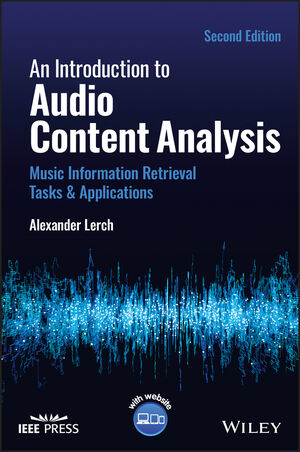
\includegraphics[scale=.20]{cover_aca2_thumb}
    %\end{flushright}
%
%\end{frame}

\begin{frame}{introduction}{music informatics group}
    \vspace{-5mm}
    \begin{columns}
    \column{.6\linewidth}
    \begin{itemize}
        %\item   \textbf{research focus}
            %\begin{itemize}
                %\item   machine learning and intelligent DSP solutions for (musical) audio 
            %\end{itemize}
        %\bigskip
        \item   \textbf{mission}
            \begin{itemize}
                \item   create new technologies transforming and improving how we \textit{make, produce, perform, discover, and consume music}
                \item   advance the field of AI for audio through \textit{knowledge-driven machine learning}
            \end{itemize}
        \bigskip
        \item   \textbf{objectives}
            \begin{itemize}
                \item   enable/improve \textit{machine understanding of music} and musical language
                \item   create \textit{interpretable and controllable systems}
                \item   design algorithms with \textit{low data requirements}
            \end{itemize}
    \end{itemize}
    \column{.4\linewidth}
        \vspace{12mm}\begin{figure}%
            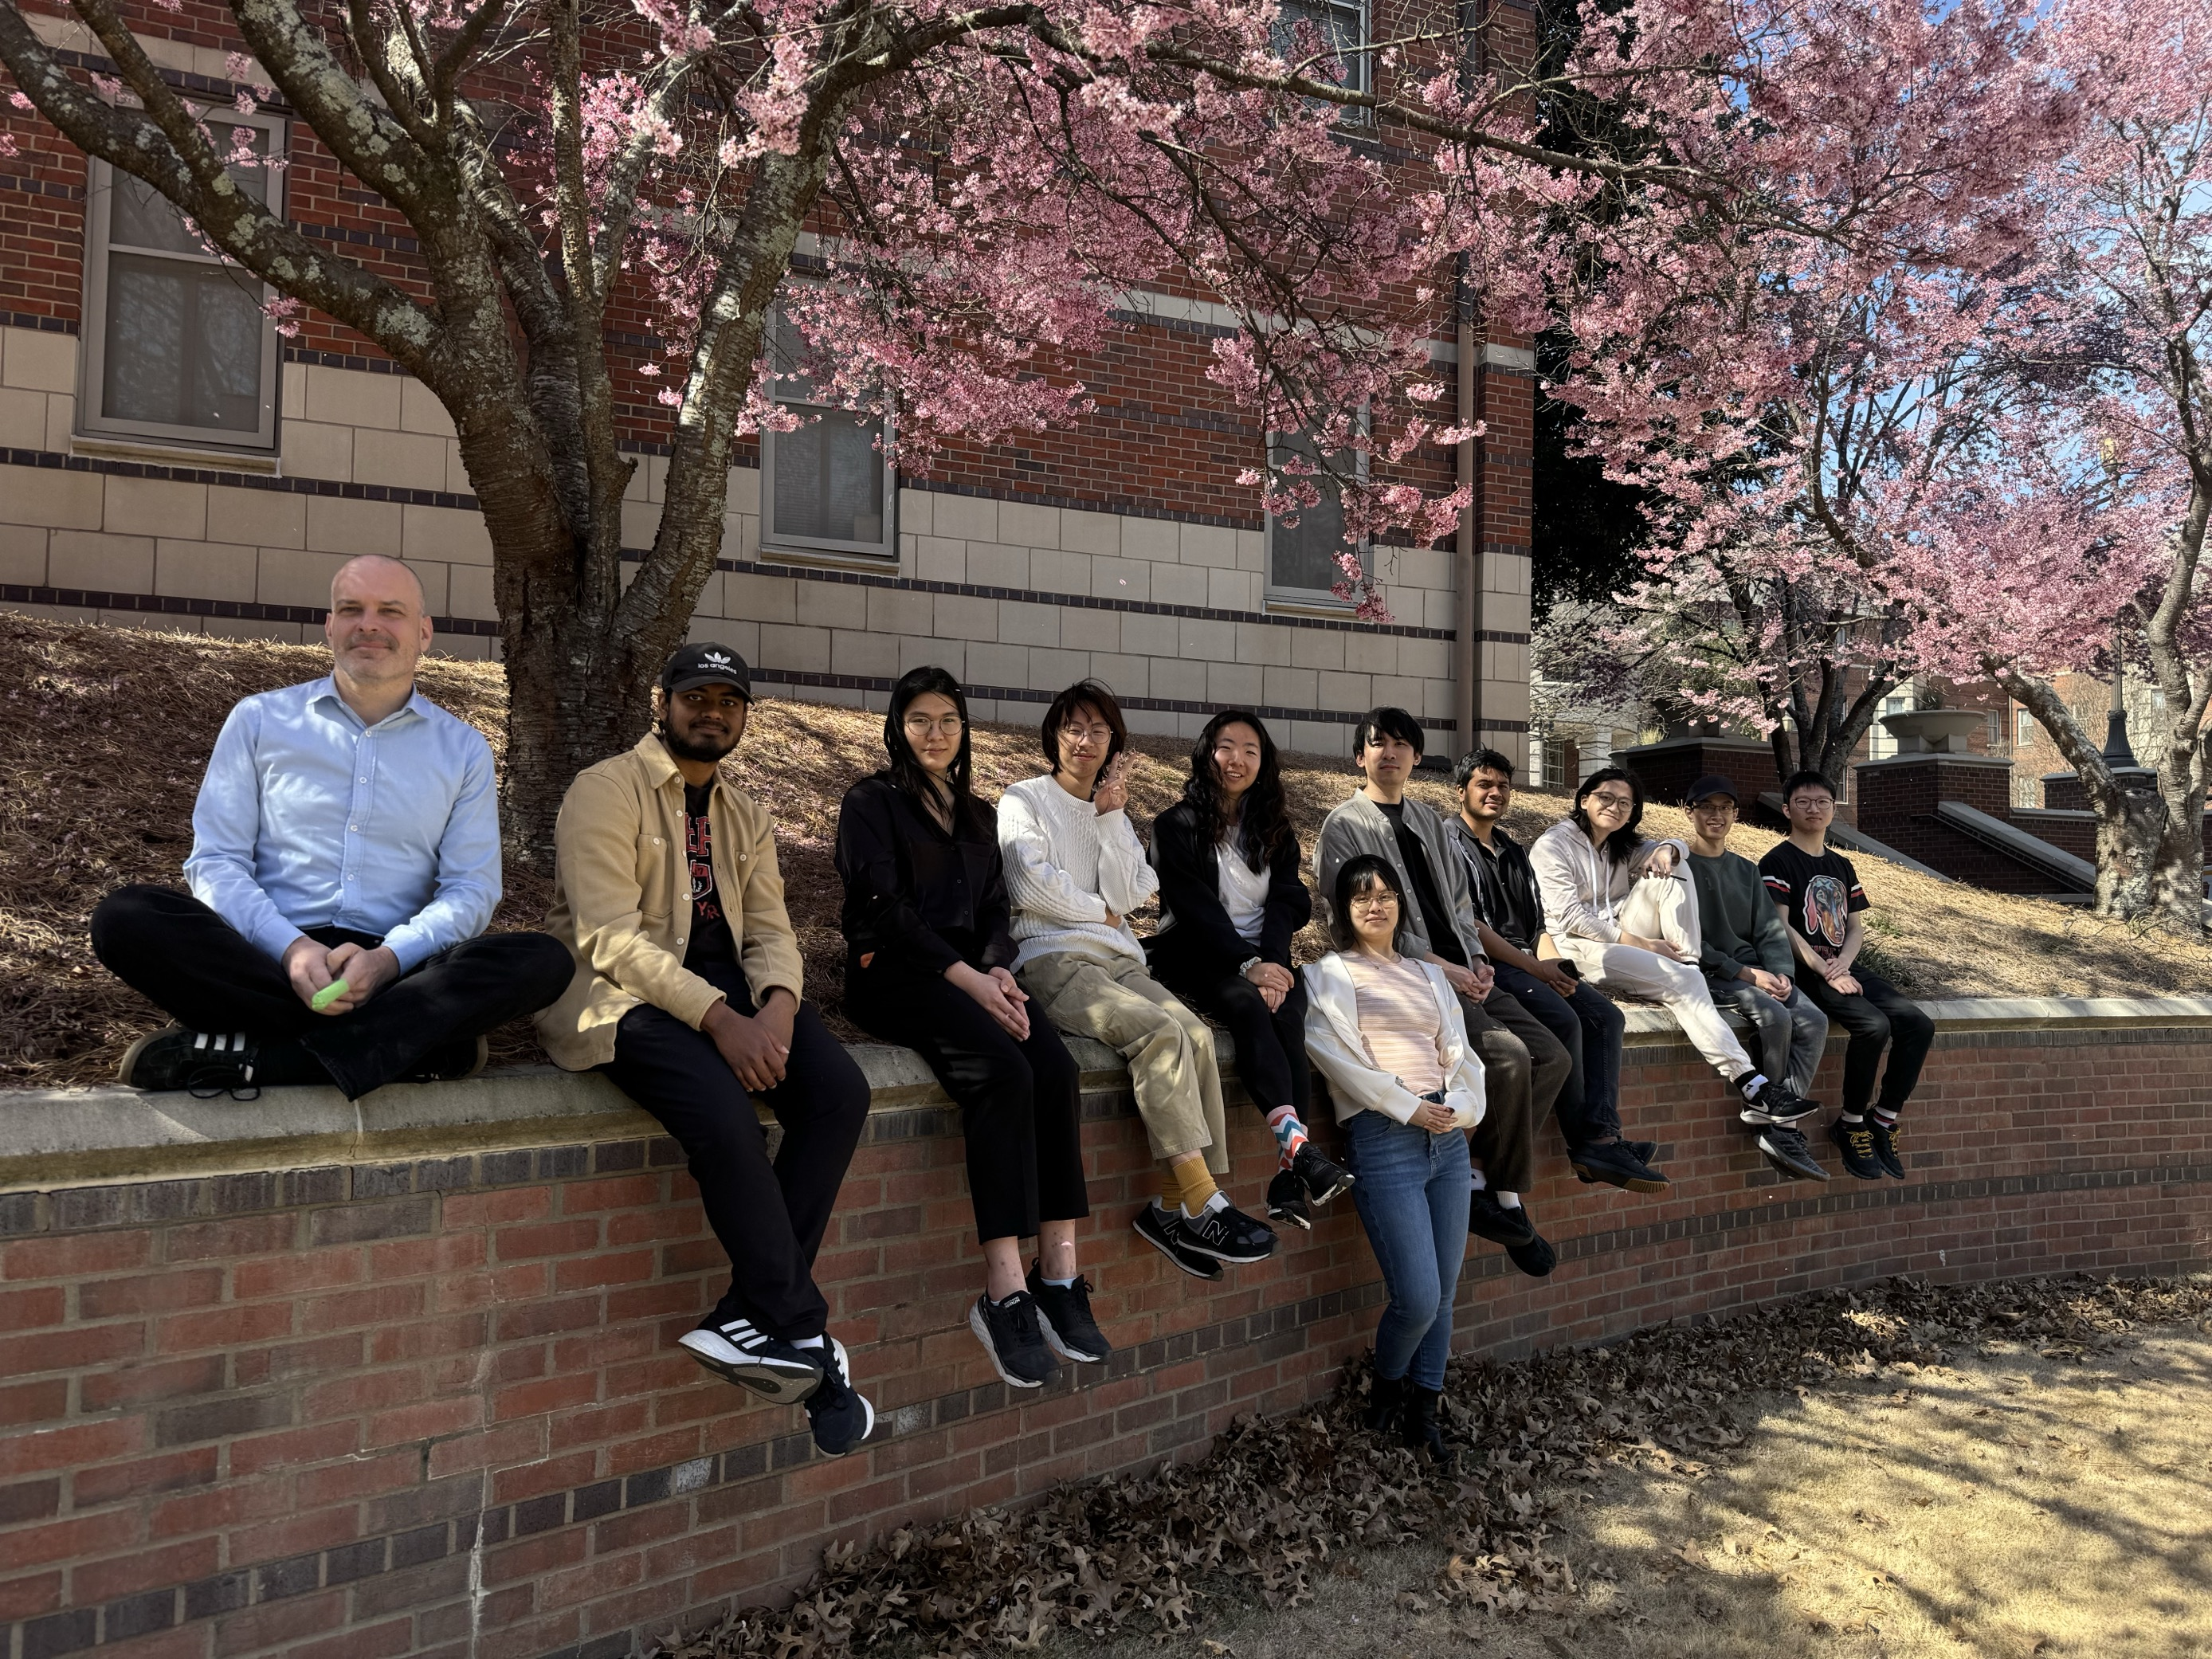
\includegraphics[width=\columnwidth]{MIG2024}%
        \end{figure}
    \end{columns}
    \addreference{\href{https://musicinformatics.gatech.edu}{musicinformatics.gatech.edu}}
    %\inserticon{person}
\end{frame}
